\documentclass{article}

% Add custom.sty from the main directory
\usepackage{../../custom}

\title{Homework 2 - Image Classification}
\author{Naomi Derel, 325324994 
\and Sagi Ben Lulu, 207031493}
\date{18.12.2024}

\begin{document}

\maketitle

%%% 1
\section{Classic Classifier}

\subsection{Loading Dataset}
The first 5 images in the CIFAR-10 dataset are shown in Figure \ref{fig:cifar10_images}.
\begin{figure}[h!]
    \centering
    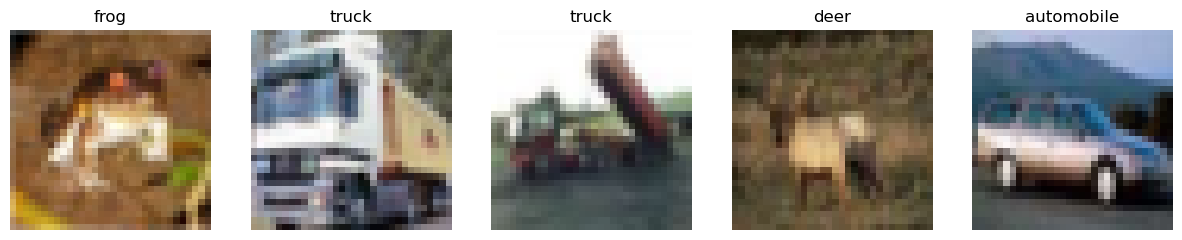
\includegraphics[width=0.8\textwidth]{figs/1.1_ex.png}
    \caption{First 5 images in CIFAR-10 dataset}
    \label{fig:cifar10_images}
\end{figure}

\subsection{K-Nearest Neighbors}
We load 10,000 samples from the training dataset, and concatenate the RGB channels of a flat image into a single vector. We then train a K-Nearest Neighbors classifier from \texttt{sklearn.neighbors} with $k=10$.

\subsection{Evaluation on Test Set}
We load 1,000 samples from the test dataset, and evaluate the classifier on the test set. The accuracy of the classifier is 0.288.
We also compute a confusion matrix between the true labels and the predicted labels, shown in Figure \ref{fig:confusion_matrix}. We note that the results are not very good, with low accuracy and many misclassifications. The best performance was achieved on the 'ship' class, which might have to do with the distinguished background color or object itself.
\begin{figure}[h!]
    \centering
    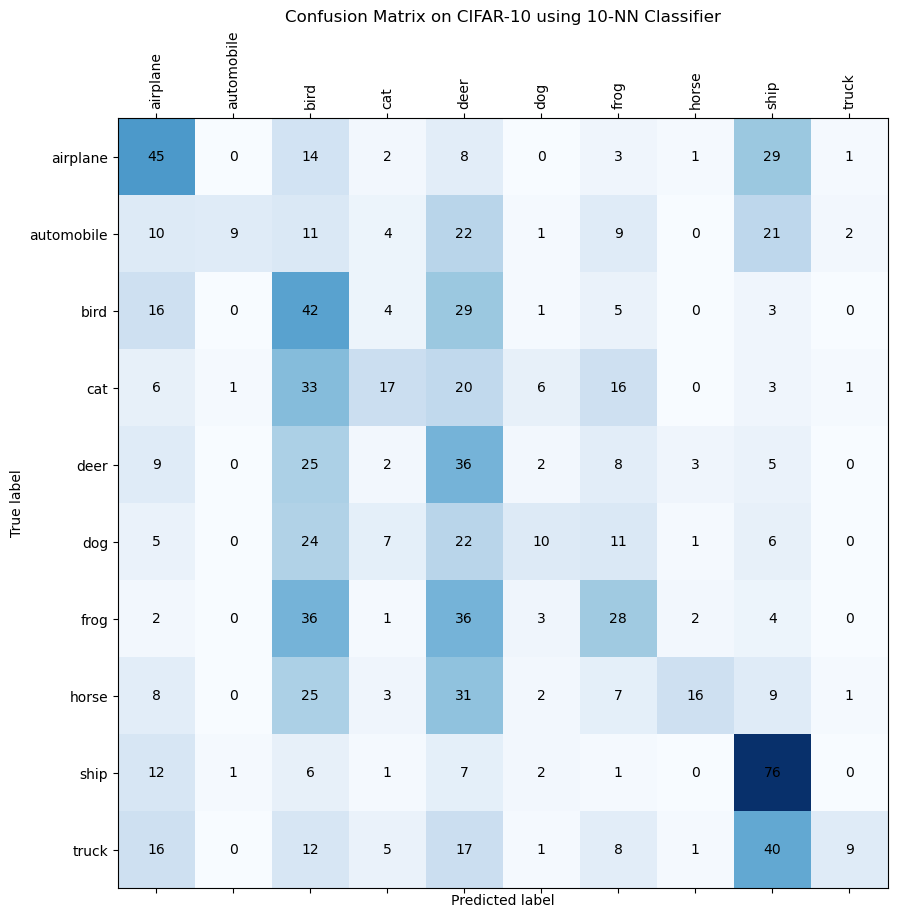
\includegraphics[width=0.7\textwidth]{figs/1.3_cm.png}
    \caption{Confusion matrix of K-Nearest Neighbors classifier}
    \label{fig:confusion_matrix}
\end{figure}

\subsection{Analysis of K Value}
The comparison of the model accuracy as a function of the number of neighbors $k$, between 1 and 30, is shown in Figure \ref{fig:k_accuracy}. We note that the accuracy is pretty low for all values of $k$ and remains below 0.3.
\begin{figure}[h!]
    \centering
    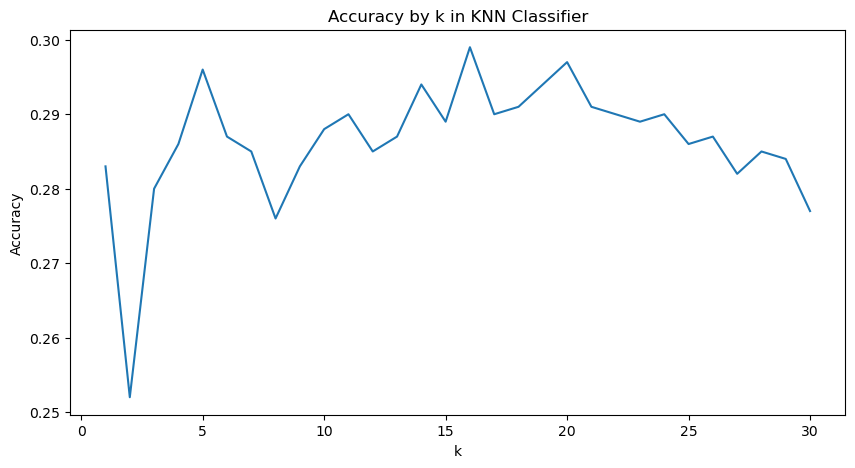
\includegraphics[width=0.7\textwidth]{figs/1.4_acck.png}
    \caption{Model accuracy as a function of the number of neighbors $k$}
    \label{fig:k_accuracy}
\end{figure}

\newpage

%%% 2
% \section{Convolution Neural Network}

% \subsection{Baseline CNN}
% We train the given CNN model with the hyper-parameters from the tutorial: learning rate of $10^{-4}$, batch size of 128, 20 epochs and the Cross-Entropy loss function.

% The baseline accuracy achieved on the test is 78.05\%. The confusion matrix in Figure \ref{fig:baseline_confusion_matrix} shows that the model performs well on all classes. The most confusion occurs between the classes 'cat' and 'dog', with the model often predicting 'cat' when the true label is 'dog'. 
% \begin{figure}[h!]
%     \centering
%     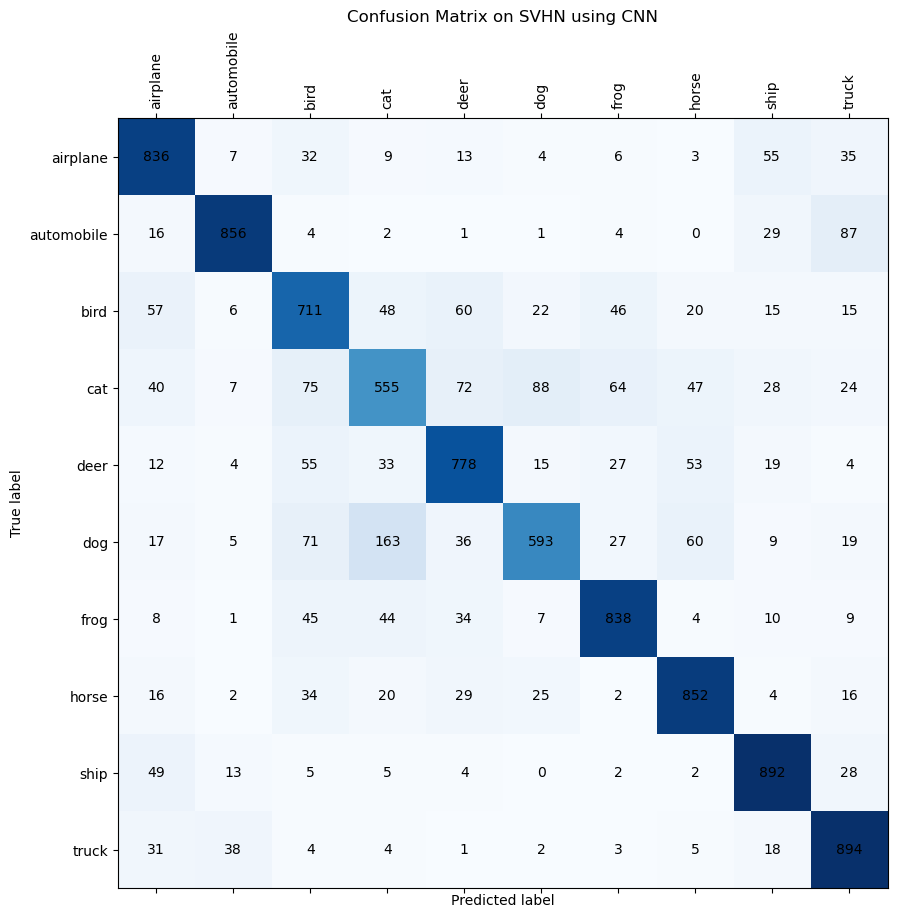
\includegraphics[width=0.7\textwidth]{figs/2.1_cm.png}
%     \caption{Confusion matrix of the baseline CNN}
%     \label{fig:baseline_confusion_matrix}
% \end{figure}

% \subsection{Designing Our Own CNN}
% We notice that the baseline model has a training accuracy of 96.576\%, much higher than the test accuracy, which indicates the model is overfitting. To address this, we expand the given architecture with more dropout and batch normalization layers.
% We also change the activation function from ReLU to LeakyReLU, which allows a small gradient when the unit is not active, and thus helps to prevent the vanishing gradient problem.

% \subsection{Training and Evaluation}

% We conduct training using the cross-validation method, allowing us early stopping by a validation set instead of overfitting, while still maintaining the same division of the data. We use the same hyper-parameters as the baseline model.

% This training results in a test accuracy of 79.29\%, which is slightly better than the baseline model. 

\newpage

%%% 3
\section{Question 3 - Foundation Models}

\subsection{Embedding Space of T-SNE}
We load all the images from the 'data/clip\_images' directory, which includes 'cats' and 'dogs' images. We then embed the images using clip, and project them using T-SNE (with random seed=18). The resulting plot is shown in Figure \ref{fig:tsne_plot}. We note that the 'cats' and 'dogs' images are well separated in the embedding space, with the 'cats' images on the right and the 'dogs' images on the left.
\begin{figure}[h!]
    \centering
    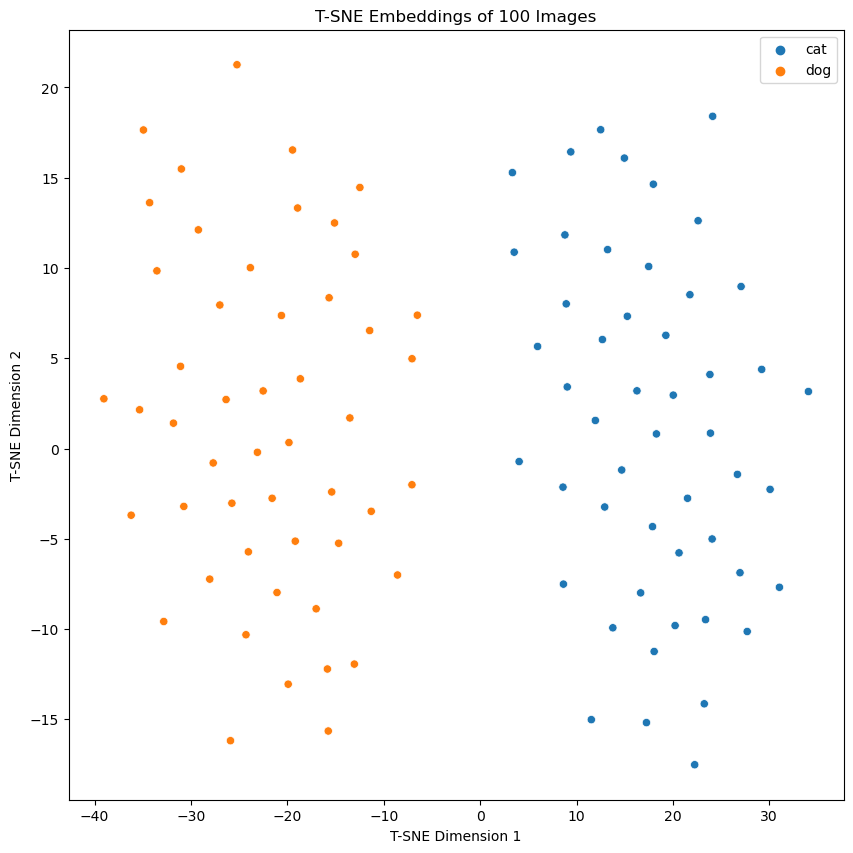
\includegraphics[width=0.6\textwidth]{figs/3.1_emb.png}
    \caption{T-SNE plot of the 'cats' and 'dogs' images}
    \label{fig:tsne_plot}
\end{figure}

\subsection{CLIP Nearest Neighbors}

We compare the image of Alfie (Figure \ref{fig:alfie}) by cosine similarity in the embeddign space (Figure \ref{fig:alfie_nn}). 

\begin{figure}[h!]
    \centering
    \begin{minipage}[b]{0.15\textwidth}
        \centering
        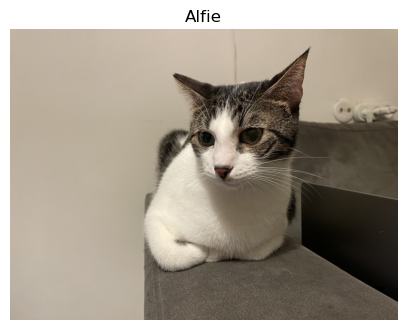
\includegraphics[width=\textwidth]{figs/3.2_alfie.png}
        \caption{Alfie}
        \label{fig:alfie}
    \end{minipage}
    \hfill
    \begin{minipage}[b]{0.75\textwidth}
        \centering
        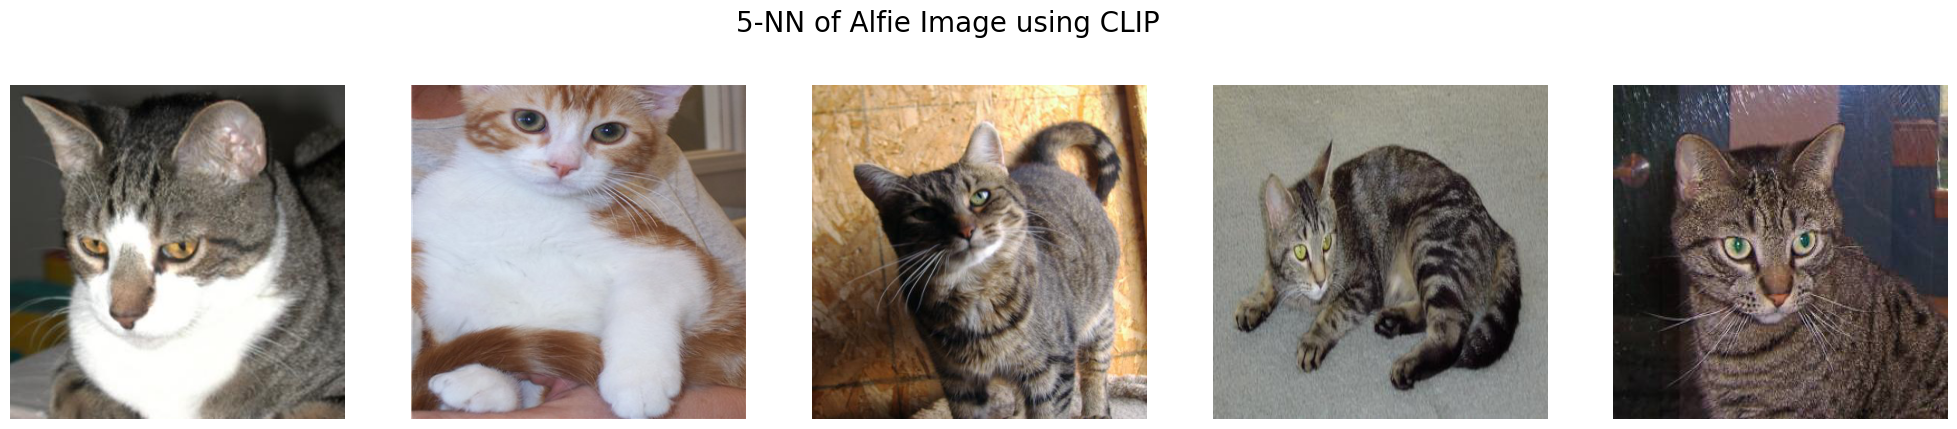
\includegraphics[width=\textwidth]{figs/3.2_5nn.png}
        \caption{5-Nearest Neighbors of Alfie in the CLIP embedding space}
        \label{fig:alfie_nn}
    \end{minipage}
\end{figure}

First, the results are all cat images and no dog images, which matches our expected result. Second, we notice that most of the cats similar coloring to Alfie (gray overall or white in the same spaces). This is a good indication that the model is able to understand the context of the image and not just the image itself.

\subsection{Classification with CLIP Textual Embeddings}
We load the images and labels from the 'data/clip\_images/test' directory.
WE embed all the images using CLIP, and create the labels: "A photo of a dog", "A photo of a cat". We embed the labels as well using the CLIP textual model. We then compute the cosine similarity between the image and the labels, and classify the image based on the label with the highest similarity. 

We achieve an accuracy of 100\% on the test set.

\subsection{Counting Objects in Images}
We write a function similar to the last step, and define the labels: "A photo of a cat", "A photo of 2 cats", "A photo of 3 cats". We then classify the images based on the label with the highest similarity. 

We succeed on 2 simple cases, with 1 and 2 cats. However, on an image with a cat and a human, we also get the prediction of 2 cats. 
This is likely due to a lack of a better label in the options we suggest as counts for cats, as the image has 2 animals.

\end{document}